% THIS IS SIGPROC-SP.TEX - VERSION 3.1
% WORKS WITH V3.2SP OF ACM_PROC_ARTICLE-SP.CLS
% APRIL 2009
%
% It is an example file showing how to use the 'acm_proc_article-sp.cls' V3.2SP
% LaTeX2e document class file for Conference Proceedings submissions.
% ----------------------------------------------------------------------------------------------------------------
% This .tex file (and associated .cls V3.2SP) *DOES NOT* produce:
%       1) The Permission Statement
%       2) The Conference (location) Info information
%       3) The Copyright Line with ACM data
%       4) Page numbering
% ---------------------------------------------------------------------------------------------------------------
% It is an example which *does* use the .bib file (from which the .bbl file
% is produced).
% REMEMBER HOWEVER: After having produced the .bbl file,
% and prior to final submission,
% you need to 'insert'  your .bbl file into your source .tex file so as to provide
% ONE 'self-contained' source file.
%
% Questions regarding SIGS should be sent to
% Adrienne Griscti ---> griscti@acm.org
%
% Questions/suggestions regarding the guidelines, .tex and .cls files, etc. to
% Gerald Murray ---> murray@hq.acm.org
%
% For tracking purposes - this is V3.1SP - APRIL 2009

\documentclass{acm_proc_article-sp}

\usepackage{url}
\usepackage{wrapfig,lipsum,cleveref}
\makeatletter
\newcommand*{\rom}[1]{\expandafter\@slowromancap\romannumeral #1@}
\makeatother
\begin{document}

\title{Prototyping of a Browser-Based Social N-Screen Platform}
\subtitle{[An Improvement of its User Experience]
}
%
% You need the command \numberofauthors to handle the 'placement
% and alignment' of the authors beneath the title.
%
% For aesthetic reasons, we recommend 'three authors at a time'
% i.e. three 'name/affiliation blocks' be placed beneath the title.
%
% NOTE: You are NOT restricted in how many 'rows' of
% "name/affiliations" may appear. We just ask that you restrict
% the number of 'columns' to three.
%
% Because of the available 'opening page real-estate'
% we ask you to refrain from putting more than six authors
% (two rows with three columns) beneath the article title.
% More than six makes the first-page appear very cluttered indeed.
%
% Use the \alignauthor commands to handle the names
% and affiliations for an 'aesthetic maximum' of six authors.
% Add names, affiliations, addresses for
% the seventh etc. author(s) as the argument for the
% \additionalauthors command.
% These 'additional authors' will be output/set for you
% without further effort on your part as the last section in
% the body of your article BEFORE References or any Appendices.

\numberofauthors{1} %  in this sample file, there are a *total*
% of EIGHT authors. SIX appear on the 'first-page' (for formatting
% reasons) and the remaining two appear in the \additionalauthors section.
%
\author{
% You can go ahead and credit any number of authors here,
% e.g. one 'row of three' or two rows (consisting of one row of three
% and a second row of one, two or three).
%
% The command \alignauthor (no curly braces needed) should
% precede each author name, affiliation/snail-mail address and
% e-mail address. Additionally, tag each line of
% affiliation/address with \affaddr, and tag the
% e-mail address with \email.
%
% 1st. author
\alignauthor
Bego\~na \'Alvarez de la Cruz\\
       \affaddr{Computer Science MSc Thesis}\\
       \affaddr{Web \& Media Group}\\
       \affaddr{Vrije Universiteit, Amsterdam}\\
       \email{begona.alvarezd@gmail.com}
}

% TO DO ABSTRACT---> LAST MORE OR LESS
\maketitle
\begin{abstract}
A second screen is a hand-device which is susceptible to provide added value to the TV content consumption. Notube, with their web browser-based second screen application, moved further through this concept, creating an assosiation between the second screen, Web and TV content. Nevertheless, the implemention still lacks completion in order achieve a full service and its users' satisfaction.
This project shows the development of a social N-Screen prototype based on previous researches and implementations carried out by Notube. This platform is intended to be used by small groups to explore on-demand content. The main goal of the project is consisted on searching and implementing features to the platform in order to offer to the final user an improved user experience. This improvement is leaded by the features that allow a completion in the user interaction flow with the platform, such as the implementation of a registration and login, the provision of persistence to the user based content and the addition of new functionalities as personal lists and likes/dislikes tracking.
\end{abstract}

\section{Introduction}

\subsection{Background}

\subsubsection{The Multi-Screen World}

The human being has become throughout the last years into a multi-screener\footnote{\textit{Multi-screening}: use of 
more than one screen at a time.} nation. From the appearance of television in our living rooms, until the incorporation of lighter and portable new devices such as smartphones or tablets, users have been including all these devices in their routines until turning them into everyday objects. Consequently, tablets, smartphones, televisions and computers has become the main group of devices with which an average user consumes most of their media content\cite{multiscreen:google}. 

\begin{figure}[!htb]
\centering
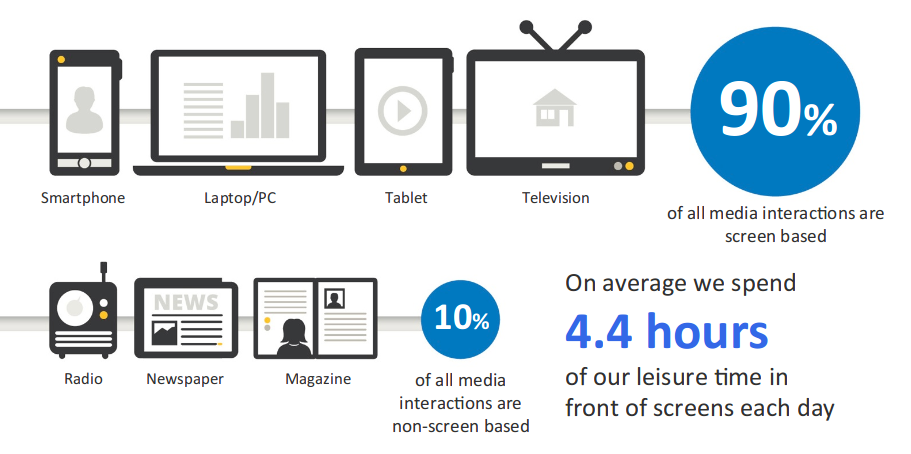
\epsfig{file=images/multiscreen-google.png, height=1.5in, width=3in}
\caption{Study of daily media interaction, obtained from \cite{multiscreen:google}}
\end{figure}

Despite each archetype provides a particular motivation and practise to users, an important fact is that screen devices as mentioned before are no longer used in isolation but collaboratively. There are two different models referring to multi-screen:  sequential and simultaneous. \textit{Sequential usage} refers to moving through more than one device in order to achieve a task. \textit{Simultaneous} concerns the usage of multiple devices at the same time for either related or unrelated activities. Both consumption forms are increasingly becoming the default mode and is surely influencing the way users engage. 

Following this scenario comes the necessity to understand how users interact with these screen devices in combination\cite{hritzuk2014multiscreen}. The opportunity to decide which device to use, where and how makes possible to users to control their own interaction and flow content. 

\begin{figure}[!htb]
	\centering
	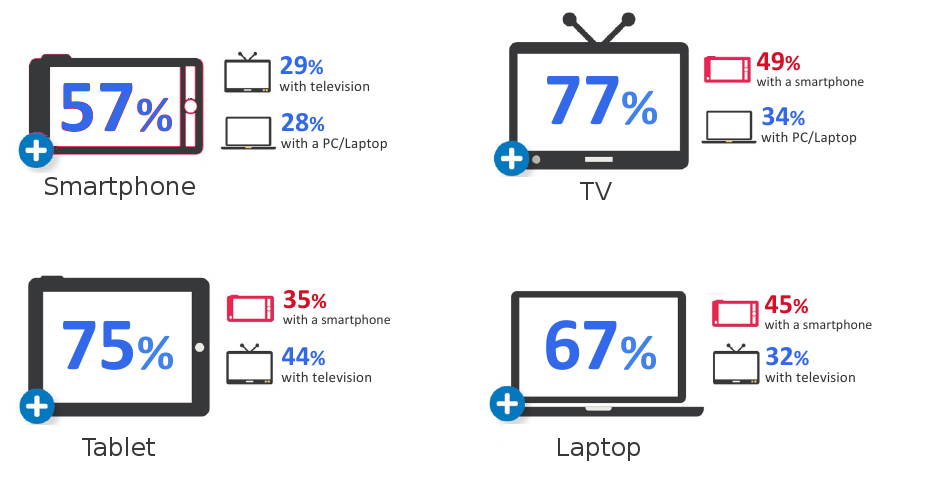
\epsfig{file=images/multi_usage2.png, height=2in, width=3.5in}
	\caption{Study of companion devices during simultaneous	 usage, obtained from \cite{multiscreen:google}}
	\label{fig:simultaneous}
\end{figure}

A Google study developed in 2012 \cite{multiscreen:google} exposed how an average consumer makes use of companion devices - smartphone, TV, tablet and laptop - during simultaneous\footnote{Usage for either related or unrelated activities.} usage - See Figure ~\ref{fig:simultaneous}. There are three main multi-screen combinations:
\begin{itemize}
  \item[-] Smartphone + TV\hspace{1.35cm}- 81\% 
  \item[-] Smartphone + Laptop/PC \hspace{0.1cm}- 66\% 
  \item[-] Laptop/PC  + TV\hspace{1.35cm} - 66\% 
\end{itemize}

Additionally, a research developed by Microsoft in 2013 \cite{microsoftcross} illustrated how is the user behaviour while multi-screening in simultaneous usage.  

\begin{itemize}
  \item[-] 68\% of consumers interact with multiple devices at the same time to access unrelated content; e.g. they may be texting a friend while watching TV. 
  \item[-] 57\% of consumers make use of more than one device simultaneously in order to achieve a related activity. 
\end{itemize}

From now on, we will focus our attention in simultaneous usage for \textit{related} activities.
 	
\subsubsection{Second Screens}

One of our everyday routines that has been altered by this new screen multitasking\footnote{\textit{Human multitasking} is the apparent performance by an individual of handling more than one task at the same time.} behaviour is that moment while a user watches TV. Viewers no longer focus their entire attention to the TV screen but share it with portable devices. 

\begin{figure}[!htb]
	\centering
	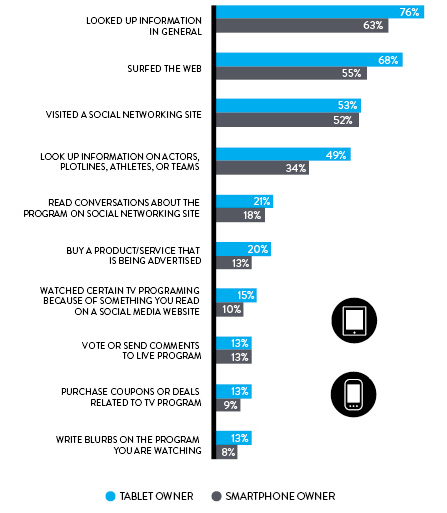
\epsfig{file=images/nielsen-tv-viewing.png, height=3.4in, width=3in}
	\caption{Tablet or smartphone activities while watching TV, obtained from \cite{nielsentv}}
	\label{fig:nielsengraph}
\end{figure}

Figure ~\ref{fig:nielsengraph} illustrates how consumers make use of their tablets and smartphones while watching TV. We can observe how indeed users not only surf on the web, but they interact with the device with activities directly related to the program or advertisement that they are watching in that moment. This demonstrates the fact that consumers are not merely interacting with their hand devices as a simple distraction, but sometimes in order to improve their TV content consumption. 

This new practice has led to the creation of the new concept \textit{second screen}. Second screen is a hand-device which is susceptible to provide added value to the TV content consumption. These devices such as tablets or smartphones play a role as companion
screens that 'connect' viewers to complementary interaction
opportunities while they watch TV via applications, additional
show-oriented content or in-synch functionalities \cite{evolumedia2}. 

This new activity has become such important that a survey developed by Nielsen Holdings N.V. \cite{nielsentv} reported 'Using a tablet or smartphone while watching TV is more common than not'. Nearly half of tablet owners - 43\%- and smartphone owners - 46\% - declared that while watching TV they are making use of their devices as second screen every day. As a consequence of this fact, there are emerging new apps\footnote{\textit{App} is an abbreviation for application. An app is a piece of software. It can run on the Internet, on a computer, on a phone or other electronic device.} which take advantage offering second screen experiences that can improve even more this interactivity while watching TV. 

Second screen apps \cite{evolumedia1} are intended to enable viewers to interact before, during and after the broadcast of a programme using a laptop, smartphone or tablet. The most competent apps, instead of distract, have the potential to increase the viewers' attention and enjoyment on the watching programme. According to \cite{evolumedia1}, eight types are distinguished in order to categorize these apps based on their functionalities: 
\begin{itemize}
  \item[-] Socializing
  \item[-] Loyalty
  \item[-] Recommendation
  \item[-] Transaction
  \item[-] Information
  \item[-] Program guides
  \item[-] Participation
  \item[-] Creation
\end{itemize}
On that account, second screen apps arised as a manner to unlock new research and business models due to the wide range of potential possibilities that offer. 

\subsubsection{Use case}

This project is developed based on an already existing platform developed by \textbf{Notube}\cite{aroyo2009notube}. Notube, is a project funded on 2009 that was specialized in second screens and Web merging. Their motivation was getting the Web and TV closer together via shared data models and content across multiple devices. They developed their own N-Screen\footnote{\textit{N-Screen} because it might be the primary screen, or one of a bunch of equals.} prototype, a Web browser-based second screen application\footnote{All the source files used to generate this application can be accessed at the public repository:
\textit{https://github.com/notube/n-screen}} for small group exploration of on-demand content, both in the same room and remotely, with each individual having their own second screen device. It integrates different combinations of recommendation strategies and allows to decide within a closed group to watch a selected program sharing a 'virtual television', that in their case is the hand device itself. 

\begin{figure}[!htb]
	\centering
	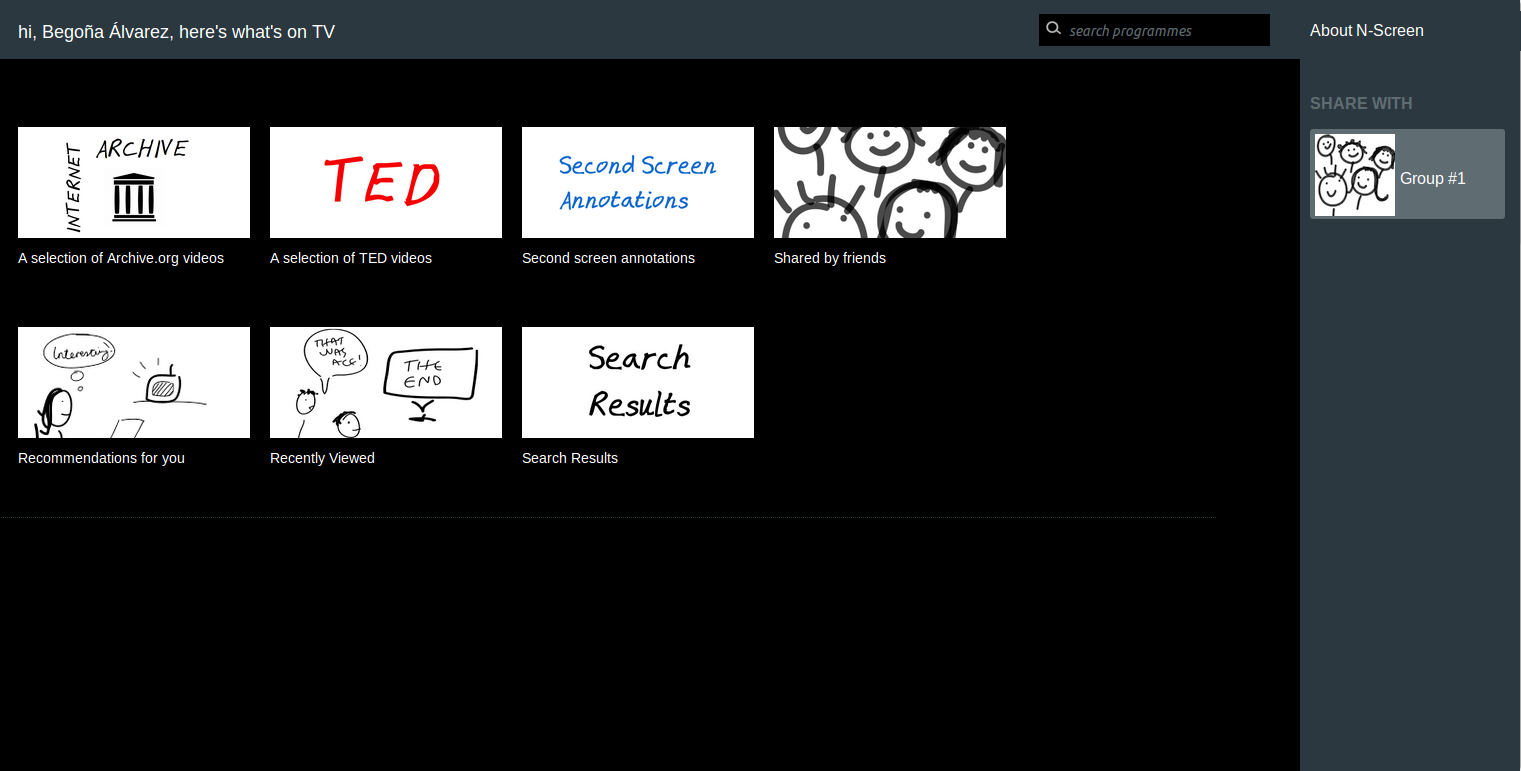
\epsfig{file=images/old_nscreen_screenshot.png, height=2in, width=3.3in}
	\caption{Notube N-Screen screenshot, source code obtained from the public repository \textit{https://github.com/notube/n-screen}}
	\label{fig:oldnotubenscreen}
\end{figure}

It is developed following a \textit{user-centric approach} in order to explore main aspects of users' content customisation demands, interaction requirements and entertainment preferences. Their main goal was to investigate if working together and collaborating to make a final decision  might help people to guide them in order to find something interesting to watch. 

\subsection{Goals}

The main goal of the project is to design and implement a browser-based\footnote{\textit{Browser-based} refers to computer tools and applications which run on a web browser via the Internet without accessing the operating system of any individual computer. These applications are accessed through web pages and can be used by people who are prevented from downloading software applications by firewalls.} second screen platform\footnote{A \textit{platform} is a group of technologies that are used as a base upon which other applications, processes or technologies are developed.}, based on the N-Screen developed by Notube, which is categorized as a social recommendation system. The implementation must meet functionality, interactivity and favourable user experience requirements. 

Most of the second screen apps in the market are not successfully developed because are focused to enhance activities  that do not fulfil the real consumer needs\cite{evolumedia1}. Consequently fail the audience engagement. This fact is crucial and it must be taken into account in order to make the platform valuable.

Furthermore, the project must accomplish certain requirements for a potential release to final users. It needs to be developed offering user based content, due to its recommendation feature. In addition, it is required to provide engaging content and interaction activities, as well as offering an intuitive appearance. Moreover, the platform must be easily adaptable, so it will not need to be entirely redone with every particular change. Hence, it is needed to reach a complete solution covering all these features, overcoming the gaps and deficiencies that other platforms show.

Here, the main goal is fragmented into more specific subgoals:

\begin{itemize}
  \item[-] \textit{Analysis of previous conclusions and results}. Study of already tested aspects. Definition of new tests to provide new data of interest. These data will help in making decisions about the implementation of interaction activities. 
  \item[-] \textit{Requirements definition}. Study of needs and constraints.
  \item[-] \textit{Back-end design}. Global design of the server requirements and new involved software. Debugging and optimization. 
  \item[-] \textit{Front-end design}. Global design of the client side requirements and new involved software. Debugging and optimization. Graphical User Interface improvement. 
  \item[-] \textit{Platform development}. Full integration of both back and front end. Development of the final demo. 
  \item[-] \textit{General purpose tests}. Tests oriented to prove the proper operation and verify
the achievement of the requirements and constraints compliance.
  \item[-] \textit{Results analysis and conclusions}. Achievement evaluation. Study of weaknesses or possible improvements. Definition of further studies.
\end{itemize}

\subsection{Project Organization}
The organization of this project is described as follows:
\begin{itemize}
  \item \textit{Analysis of previous conclusions and results}. 
  
  At this first stage, N-Screen-related information and specific knowledge was acquired. An approach to the development tools was also outlined. Goals:
  \begin{itemize}
  	\item [-]Second screen state-of-the-art review. Review of the current commercial
solutions.
	\item [-]Adaptation to the development of the platform as well as required tools (repository, client and server side programming languages research and learning, etc\dots).
	\item [-]Analysis of related projects results, either completed or under development. 
  \end{itemize}
  
  \item \textit{Software design}.
  
  This phase covered from the first software definitions and  specifications, to the platform implementation until reaching a final demo. Goals:

  \begin{itemize}
  	\item [-]Back-end design and implementation for required features.
	\item [-]Front-end design and implementation for required features.
	\item [-]Content dataset migration. 
	\item [-]Back and front end integration. Source code
debugging and improvement. 
  \end{itemize}
	
  \item \textit{Tests and evaluation}. 
  
  At last, the final demo was evaluated and the results were analyzed. Goals:
  
  \begin{itemize}
  	\item [-]Fully integrated back-end and front-end test.
	\item [-]Interaction test.
	\item [-]Graphical user interface test.
	\item [-]User experience test.
	\item [-]Results interpretation and conclusions review. Statement of further studies and future development lines. Found problems evaluation.
  \end{itemize}
  
  \item \textit{Documentation generation}.
  
  Dissertation and other required documentation writing. 
\end{itemize}


\subsection{Outline}
Typically, the body of a paper is organized
into a hierarchical structure, with numbered or unnumbered
headings for sections, subsections, sub-subsections, and even
smaller sections.  The command \texttt{{\char'134}section} that
precedes this paragraph is part of such a
hierarchy.\footnote{This is the second footnote.  It
starts a series of three footnotes that add nothing
informational, but just give an idea of how footnotes work
and look. It is a wordy one, just so you see
how a longish one plays out.} \LaTeX\ handles the numbering
and placement of these headings for you, when you use
the appropriate heading commands around the titles
of the headings.  If you want a sub-subsection or
smaller part to be unnumbered in your output, simply append an
asterisk to the command name.  Examples of both
numbered and unnumbered headings will appear throughout the
balance of this sample document.


\section{State-of-Art}
Typically, the body of a paper is organized
into a hierarchical structure, with numbered or unnumbered
headings for sections, subsections, sub-subsections, and even
smaller sections.  The command \texttt{{\char'134}section} that
precedes this paragraph is part of such a
hierarchy.\footnote{This is the second footnote.  It
starts a series of three footnotes that add nothing
informational, but just give an idea of how footnotes work
and look. It is a wordy one, just so you see
how a longish one plays out.} \LaTeX\ handles the numbering
and placement of these headings for you, when you use
the appropriate heading commands around the titles
of the headings.  If you want a sub-subsection or
smaller part to be unnumbered in your output, simply append an
asterisk to the command name.  Examples of both
numbered and unnumbered headings will appear throughout the
balance of this sample document.


\section{Review Study}
A model for the platform is defined in this chapter. Initially, the first version of the N-Screen developed by Notube\cite{aroyo2009notube} is evaluated to obtain some guidelines and potential improvements facing our own. The final software implementation requirements and constraints are defined. Finally, a discussion and evaluation over different features is carried out, exposing different options and some final conclusions in order to face a potential deployment to final users.
\subsection{Browser-Based Social N-Screen Platform Model}

Essentially, the BBSNSP\footnote{Browser-Based Social N-Screen Platform} responds to second screen application based on a recommendation system. However, a further review shows some general differences:

\begin{itemize}
  	\item [-]\textit{Browser-based}: instead of being developed as a mobile or computer app, the BBSNS is a web app. A \textit{web app} refers to software that runs on a web browser. This way, not only the app can be updated and maintained without disturbing potential users by requiring them to re-download. Additionally, it provides implicit support for cross-platform\footnote{\textit{Cross-platform} regards the capability of a software to run identically on different platforms.} compatibility. 
	\item [-]\textit{Group decision recommendation system}. The recommendation feature is focused on 'how collaborating together might help people find something interesting to watch'\footnote{https://notube3.wordpress.com/2011/10/10/n-screen-a-second-screen-application-for-small-group-exploration-of-on-demand-content/}. It is designed to be used within a small group of friends in a collaboratively way to reach together a successful programme to watch. 
	\item [-]\textit{Apart\footnote{Different physical locations.} group oriented}: this BBSNS is mainly designed to watch together with other friends but being remotely located. 
	\item [-]\textit{N-Screen}: It is not only oriented to be used as a secondary. It is considered that it might be used as a primary screen, secondary screen, or one of a screen devices collection. 
\end{itemize}

\subsection{First Browser-Based Social N-Screen Platform Review}

The first BBSNSP was a project of Notube developed in 2011. It supposed a big step forward to get the Web and TV closer together using shared data models and content across multiple devices\cite{schopman2010notube}. It is designed to help deciding and enabling to interact using drag and drop over screen devices. It allowed to investigate  how helpful is group collaboration in order to find an interesting programme to watch, for limited group of users. It gave the strengths and weaknesses to establish the fundamentals for future developments.

While constituting a successful platform meeting most of its features, the Notube BBSNSP introduced some issues found after its evaluation. This issues are following listed. 

\rom{1}) As a recommender system, the platform is intended to be user based content oriented. User preferences and explicit interaction should provide to the recommendation strategies an on-real-time update to re-rank the displayed personal suggestions\cite{libbyrecommender}. In Notube's platform, user interaction is treated as \textit{volatile} data, each time that the session is closed, the information is lost. This implementation impedes to exploit all this relevant information. Figure~\ref{fig:recomm} shows the 5 tasks that are intended to be accomplished by the recommendation engines in the client-side. If the platform lacks tracking of user interaction and preferences, it would not be possible to realize properly the first \textit{traing} step due to a lack of information.

\begin{figure}[!htb]
\centering
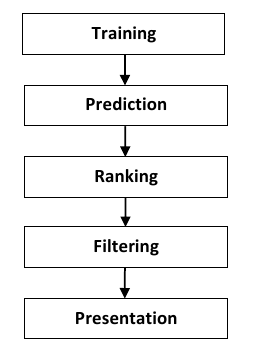
\epsfig{file=images/recommender_tasks.png, height=2in, width=1.5in}
\caption{Recommender system tasks, obtained from \cite{libbyrecommender}}
\label{fig:recomm}
\end{figure}

\rom{2}) Their own preliminary findings after the evaluation\footnote{https://notube3.wordpress.com/2011/12/12/preliminary-findings-of-n-screen-user-testing/} showed us a weak point. Notube results obtained after testing N-Screen with real users showed how some of them received a successful recommendation and indeed were wishing to watch later that specific selected programme. They received feedback such as ''Not for watching something instantly, only for making suggestions for things that could choose to watch later if you wanted to'' or ''I do not think it is on to recommend things for others to watch instantly''. This results revealed an interesting \textit{sequential usage} behaviour. In this case, instead of passing from one device to another, the user is making use of the same device time later to accomplish a task. Therefore, not only the volatile activity of the user, but also a lack of option to save wished programmes for a future moment, makes unlikely the activity to watch \textit{that programme later}. 

\rom{3}) It is very important to offer an attractive set of possible activities for the user to interact with the \cite{skadberg2004visitors}. The only implicit offered interactions are the browsing and the suggestion part. For this reason, we found that Notube N-Screen slightly incomplete in terms of interactivity actions. 

\rom{4}) The platform was designed to be not only a recommendation system, but also a place to watch a selected programme. There exist two different ways to realize this action: locally and remotely. 
The first one is performed when a user decides to watch a programme individually. By contrast, the second one is conducted when a group decides to watch together a selected programme and the members are located in remote locations. This last visualization mode involves the execution of a browser-based 'virtual TV' in which every person within the group can watch simultaneously the same. Unfortunately,  this last feature was not working because the programme visualization part was missing. Making the virtual TV feature working is indeed necessary for a complete success of the platform. 


\section{Implementation Study}
Typically, the body of a paper is organized
into a hierarchical structure, with numbered or unnumbered
headings for sections, subsections, sub-subsections, and even
smaller sections.  The command \texttt{{\char'134}section} that
precedes this paragraph is part of such a
hierarchy.\footnote{This is the second footnote.  It
starts a series of three footnotes that add nothing
informational, but just give an idea of how footnotes work
and look. It is a wordy one, just so you see
how a longish one plays out.} \LaTeX\ handles the numbering
and placement of these headings for you, when you use
the appropriate heading commands around the titles
of the headings.  If you want a sub-subsection or
smaller part to be unnumbered in your output, simply append an
asterisk to the command name.  Examples of both
numbered and unnumbered headings will appear throughout the
balance of this sample document.

\section{Evaluation and Results}
Typically, the body of a paper is organized
into a hierarchical structure, with numbered or unnumbered
headings for sections, subsections, sub-subsections, and even
smaller sections.  The command \texttt{{\char'134}section} that
precedes this paragraph is part of such a
hierarchy.\footnote{This is the second footnote.  It
starts a series of three footnotes that add nothing
informational, but just give an idea of how footnotes work
and look. It is a wordy one, just so you see
how a longish one plays out.} \LaTeX\ handles the numbering
and placement of these headings for you, when you use
the appropriate heading commands around the titles
of the headings.  If you want a sub-subsection or
smaller part to be unnumbered in your output, simply append an
asterisk to the command name.  Examples of both
numbered and unnumbered headings will appear throughout the
balance of this sample document.

\section{Conclusions}
This paragraph will end the body of this sample document.
Remember that you might still have Acknowledgments or
Appendices; brief samples of these
follow.  There is still the Bibliography to deal with; and
we will make a disclaimer about that here: with the exception
of the reference to the \LaTeX\ book, the citations in
this paper are to articles which have nothing to
do with the present subject and are used as
examples only.
%\end{document}  % This is where a 'short' article might terminate

%ACKNOWLEDGMENTS are optional
\section{Acknowledgments}
This section is optional; it is a location for you
to acknowledge grants, funding, editing assistance and
what have you.  In the present case, for example, the
authors would like to thank Gerald Murray of ACM for
his help in codifying this \textit{Author's Guide}
and the \textbf{.cls} and \textbf{.tex} files that it describes.

%
% The following two commands are all you need in the
% initial runs of your .tex file to
% produce the bibliography for the citations in your paper.
\bibliographystyle{abbrv}
\bibliography{sigproc}  % sigproc.bib is the name of the Bibliography in this case
% You must have a proper ".bib" file
%  and remember to run:
% latex bibtex latex latex
% to resolve all references
%
% ACM needs 'a single self-contained file'!
%
%APPENDICES are optional
%\balancecolumns
\appendix
%Appendix A
\section{Headings in Appendices}
The rules about hierarchical headings discussed above for
the body of the article are different in the appendices.
In the \textbf{appendix} environment, the command
\textbf{section} is used to
indicate the start of each Appendix, with alphabetic order
designation (i.e. the first is A, the second B, etc.) and
a title (if you include one).  So, if you need
hierarchical structure
\textit{within} an Appendix, start with \textbf{subsection} as the
highest level. Here is an outline of the body of this
document in Appendix-appropriate form:
\subsection{Introduction}
\subsection{The Body of the Paper}
\subsubsection{Type Changes and  Special Characters}
\subsubsection{Math Equations}
\paragraph{Inline (In-text) Equations}
\paragraph{Display Equations}
\subsubsection{Citations}
\subsubsection{Tables}
\subsubsection{Figures}

\subsubsection{Theorem-like Constructs}
\subsubsection*{A Caveat for the \TeX\ Expert}
\subsection{Conclusions}
\subsection{Acknowledgments}
\subsection{Additional Authors}
This section is inserted by \LaTeX; you do not insert it.
You just add the names and information in the
\texttt{{\char'134}additionalauthors} command at the start
of the document.
\subsection{References}
Generated by bibtex from your ~.bib file.  Run latex,
then bibtex, then latex twice (to resolve references)
to create the ~.bbl file.  Insert that ~.bbl file into
the .tex source file and comment out
the command \texttt{{\char'134}thebibliography}.
% This next section command marks the start of
% Appendix B, and does not continue the present hierarchy
\section{More Help for the Hardy}
The acm\_proc\_article-sp document class file itself is chock-full of succinct
and helpful comments.  If you consider yourself a moderately
experienced to expert user of \LaTeX, you may find reading
it useful but please remember not to change it.
\balancecolumns
% That's all folks!
\end{document}
